\chapter{Übersicht Stand der Forschung / Technik} 
\label{chapter:Kapitel4}
\lhead{Kapitel 4. \emph{Übersicht Stand der Forschung / Technik}} 

Das vorliegende Kapitel stellt Technologie und Konzepte vor, welche den Stand der Technik und Forschung im Bereich der PLE-Entwicklung darstellen oder notwendig sind, um die in Kapitel \ref{chapter:Kapitel3} entwickelnden Anforderungen an eine webbasierte und offline fähige Personal Learning Environment zu erfüllen. Eröffnet wird das Kapitel wird mit einem Blick auf zwei unterschiedliche Konzepte zum Aufbau und zur Klassifikation von PLEs, welchem bei dem Design und der Evaluierung des Systems von Nutzen sind. Anschließend werden die aktuell verbreitetsten Widget-Frameworks beschrieben. Es folgen zwei Abschnitte zu dem technologischen Fundament, des Systems. Das Kapitel schließt mit einem Abschnitt über die Verwendung des Prototypen auf einem USB-Stick und einem kurzen Überblick über ähnliche auf dem Markt befindliche Systeme. 

\section{Konzepte zum Aufbau und zur Klassifikation von PLEs}
Das Ziel dieser Arbeit ist der Entwurf und die prototypische Implementierung einer Personal Learning Environment. Zum Erreichen dieses Zieles ist es hilfreich sich einen Rahmen zu schaffen, in dem diese Implementierung stattfinden kann. Ein solcher Rahmen kann helfen ein Vokabular zu erstellen, auf dessen Basis die benötigten Funktionalitäten der PLE  beschrieben und kategorisiert werden können. Zur Schaffung dieses Rahmens wurden für diese Arbeit zwei Konzepte gewählt, welche auf Basis unterschiedlicher Ansätze Funktionalitäten von PLEs auf unterschiedliche Klassen abbilden. Zum einen gibt es den Versuch von Palmér Dimensionen zu definieren und die Funktionalitäten von PLEs diesen Dimensionen zuzuordnen. Palmér schafft damit ein System, um unterschiedliche PLE-Systeme kategorisieren zu können. Zum anderen definiert Wilson Entwurfsmuster für Personal Learning Environments. Diese Muster sollen helfen wiederkehrende Konzepte beim Entwurf einer PLE zu beschreiben und Lösungsansätze für häufig auftretende Probleme zu bieten. Diese beiden Konzepte werden im Folgenden vorgestellt. Anschließend wird unter Bezugnahme auf die Anforderungsanalyse begründet auf welchen Teilen der Schwerpunkt bei der Umsetzung dieser Arbeit liegt.

\subsection{Dimensionen nach Palmér}\label{section:dimensions_palmer} 
Palmér definiert sechs Dimensionen mit denen er so viele relevanten Funktionalitäten von PLEs wie möglich erfassen möchte (vgl. \cite{Palmer2009}). Trotz dessen sollen diese Dimensionen relativ unabhängig voneinander sein, so dass es möglich ist das unterschiedliche Plattformen einige Dimensionen mehr und andere weniger berücksichtigen und implementieren. Eine PLE kann dann Anhand des Grades ihrer Implementierung der einzelnen Dimensionen kategorisiert und bewertet werden.
\begin{enumerate}
 \item \emph{Screen-Dimension}: Die Screen-Dimension befasst sich mit Aspekten, welche die Darstellungsebene von PLEs definieren. Hierzu zählt Palmér insbesondere das User-Interface und die Usability des PLE-Containers (wie sind die Widgets angeordnet, wie können neue Widgets gesucht und hinzugefügt werden, wie einfach kann sich der Nutzer im System bewegen etc.), welcher als Einstiegspunkt in die Systembedienung dient und das User-Interface der einzelnen Widgets. Es gehören aber auch Funktionalitäten wie die Möglichkeit Inhalte und Ressourcen mit anderen Nutzern zu teilen und die Integration der selben Widgets in unterschiedlichen PLE-Containern zu der Screen-Dimension.
 \item \emph{Data-Dimension}: Mit der Data-Dimension beschreibt Palmér Funktionalitäten, die für die Portabilität der verwendeten Daten innerhalb einer PLE notwendig sind. Idealerweise sollen Widgets in der Lage sein untereinander und mit dem PLE-Container zu kommunizieren. Sie sollen Daten austauschen können und sich so weit wie möglich über ihre Zustände informieren. Des Weiteren soll es möglich sein die Daten der Widgets zu exportieren und sie an anderer Stelle oder in einem anderen PLE-Container wieder zu importieren und weiterzuverwenden. Mit der fortschreitenden Mobilität der Nutzer wird es immer wichtiger, dass der Zugriff auf die PLE auch dann möglich ist, wenn kein Zugriff auf das Internet besteht. Somit ist es nicht nur notwendig Daten zu importieren und zu exportieren, sondern auch zwischen einem Offline und einem Online-Speicher zu synchronisieren, sobald eine entsprechende Zustandsänderung eintritt.
 \item \emph{Social-Dimension}: Ein wesentlicher Bestandteil des Web 2.0 ist die Vernetzung von Freunden und Menschen mit ähnlichen Interessen untereinander. Dem trägt Palmér mit der Social-Dimension Rechnung. Diese Dimension gibt an, wie sehr eine PLE Funktionalitäten sozialer Netzwerke wie Freundeslisten integriert und Möglichkeiten bietet den Zugriff auf geteilte Ressourcen auf bestimmte Typen von Freunden einzuschränken. Palmér zählt aber auch die Möglichkeit zur Erstellung von eigenen offenen oder geschlossenen Lerngruppen zu Funktionalitäten, die in diese Dimension fallen.
 \item \emph{Temporal-Dimension}: Die in der Screen- und der Social-Dimension beschriebene Kollaboration zwischen Nutzern der PLE bringt neue Anforderungen mit sich. So ist es beispielsweise notwendig oder zumindest wünschenswert, dass geänderte Inhalte sich in Echtzeit in den Instanzen der Widgets manifestieren, die ebenfalls auf diese Inhalte zugreifen. Hierbei sollten auch Probleme, wie auftretende Konflikte bei gleichzeitigem Bearbeiten der selben Ressource in Betracht gezogen werden.
 \item \emph{Activity-Dimension}: Die Activity-Dimension beschreibt die Möglichkeit Abläufe und Workflows innerhalb einer PLE aktiv zu gestalten. Hierzu gehören unterer anderem einfache Dinge wie Anleitungen als Hilfestellung für den Nutzer zur Bewegung innerhalb der PLE. Besonderen Wert legt Palmér aber auf die Abbildung von Lernsequenzen innerhalb der PLE. So können bestimmte Widgets auf bestimmte Ereignisse reagieren oder sich selbst aktivieren oder deaktivieren. Des Weiteren können unterschiedlichste Konzepte aus dem Bereich des E-Learnings wie zum Beispiel \href{http://www.imsglobal.org/learningdesign/}{IMS Learning Design}\footnote{\url{http://www.imsglobal.org/learningdesign/}} oder \href{http://ltsc.ieee.org/wg12/files/LOM_1484_12_1_v1_Final_Draft.pdf}{Learning Object Metadata (LOM)}\footnote{\url{http://ltsc.ieee.org/wg12/files/LOM_1484_12_1_v1_Final_Draft.pdf}}) in den Widgets oder dem PLE-Container selber implementiert werden.
 \item \emph{Runtime-Dimension}: Die Runtime-Dimension befasst sich mit Funktionalitäten, die die Interoperabilität zwischen PLE-Systemen und Komponenten beinhalten. Nach Palmér werden Nutzer in der Zukunft nicht nur eine PLE benutzen, sondern je nach Bedürfnis oder Anwendungsfall zwischen ihnen hin- und herwechseln. Hierfür sollte es möglich sein Importe und Exporte für Inhalte und Einstellungen sowohl der einzelnen Widgets als auch des PLE-Containers vorzunehmen. Damit eine Interoperabilität
 zwischen PLEs möglich wird, ist es notwendig, dass Standards geschaffen werden, welche von den unterschiedlichen PLEs anerkannt und implementiert werden. Zusätzlich gehört für Palmér auch die Möglichkeit der Einbettung und Kommunikation von PLEs in und mit größeren Systemen zu dieser Dimension.
\end{enumerate}

\subsection{Muster für das Design von Personal Learning Environments}\label{section:wilson_patterns}
\cite{Wilson2008} stellt unterschiedliche Muster vor, die bei der Entwicklung einer PLE helfen sollen. Hierbei legt er seinen Fokus auf die dezentralisierte  nutzerzentrierte Natur von PLEs. Als Motivation dafür gibt er an, dass PLEs nicht ein einfaches Stück Software seien. Vielmehr stellen sie eine Umgebung dar, in der Menschen mit Werkzeugen, Ressourcen und Communities in einer lockeren und nicht vorher strikt fixierten Art und Weise kommunizieren. Dieser lockere Aufbau macht es für den Entwickler jedoch nicht leichter ein für den Anwender gut nutzbare Systeme zu entwerfen. Wilson leitet seine Muster von denen ab, die von der Universität von Bolton während des "`Personal Learning Environments Reference Model Project"' Projektes entwickelt wurden. Er versucht die Anzahl der Muster jedoch von ursprünglich 77 deutlich zu reduzieren, indem er Muster, die sich auf einfache Funktionen beziehen zu größeren Gruppen zusammenfasst und so eher allgemeine Charakteristika von PLEs beschreibt.

Wilson unterscheidet zwischen zwei verschiedenen Arten von Mustern für PLEs: Muster für persönliche Anwendungen (Personal Tools) und Muster für Lernnetzwerke (Learning Networks). Personal Tools stellen hierbei die Werkzeuge dar, die ein Nutzer direkt für seine Lernaktivitäten nutzt. Er interagiert mit unterschiedlichen sozialen Netzen (zum Beispiel Lernnetzwerken) oder verwendet die Tools anderweitig für seine persönliche Art des Lernens. 
Wilson definiert Learning Networks als die Infrastruktur, welche notwendig ist um Lernnetzwerke mit Hilfe sozialer Netze oder Communities aufzubauen. Des Weiteren zählt er auch die Menge der Online-Services hinzu, welche von einem Lehrinstitut den Lernenden zur Verfügung gestellt werden (vgl. \cite{Wilson2008}).

Diese Arbeit beschäftigt sich mit dem Aufbau einer PLE, welche direkt vom Nutzer für seine Lernaktivitäten verwendet wird. Learning Networks spielen hierfür keine oder eine nur sehr untergeordnete Rolle, so dass die Muster für das Erstellen eben dieser hier nicht weiter beleuchtet werden. Im Folgenden werden die Muster für Personal Tools vorgestellt. Diese ähneln meist einer Empfehlung, wie eine bestimmte Funktion umgesetzt werden sollte oder welche Funktionalitäten vorhanden sein sollten, um die Erfahrung des Nutzers im Umgang mit dem System zu verbessern.

\begin{enumerate}
 \item \emph{Discourse Monitor}\label{wilson_patterns:discourse_monitor}: In einer PLE werden Informationen aus potentiell sehr vielen und unterschiedlichen Quellen verarbeitet. Um dem Nutzer die Möglichkeit zu geben wichtige Informationen schneller herauszufiltern oder zu priorisieren, sollte ein Discourse Monitor implementiert werden. Dieser fasst die wichtigsten Informationen aus den unterschiedlichen Quellen zusammen und bereitet sie in übersichtlicher Art und Weise auf. Dem Nutzer soll es dann möglich sein, die dargestellten Daten zu Filtern, zu priorisieren, seine Favoriten zu kennzeichnen oder neu eingetroffene Daten einfach und zeitnah zu erkennen. 
 \item \emph{Connection Hub}: Der Nutzer einer PLE ist bei verschiedensten Netzwerken angemeldet und hat dort höchstwahrscheinlich unterschiedliche Informationen hinterlegt. Es ist auch möglich, dass eine Kommunikation über Netzwerkgrenzen hinweg stattgefunden hat. Diese Daten sind meist nicht in einem einzigen Netzwerk darstellbar. Ein Connection Hub soll in der Lage sein oder den Nutzer in die Lage versetzen diese Verbindungen darzustellen und aufzubereiten. Es wäre beispielsweise vorstellbar, dass es dem Nutzer ermöglicht wird Informationen und Daten verschiedenster Netzwerke zu kombinieren ohne, dass diese Netzwerke direkt in Kontakt zueinander stehen.
 \item \emph{Create and Mix Media}: Es ist unabdingbar, dass während des computergestützten Lernens sowohl von dem Lernenden, als auch von dem Lehrenden Ressourcen erstellt und diese auch anderen zur Verfügung gestellt werden. Hierzu gehören alle Arten von Ressourcen, also Textdateien, Notizen, Quellcode, Videos, Bilder, Präsentationen etc.. Die PLE sollte es dem Nutzer ermöglichen diese Ressourcen zu erstellen (auch unter Zuhilfenahme externer Services) und diese dann an unterschiedliche Netzwerke zu verteilen. 
 \item \emph{Integrate Identities}: Durch das Nutzen unterschiedlicher Services hat der Nutzer höchstwahrscheinlich auch Useraccounts bei all diesen Services erstellt. Wilson schlägt für die Vereinfachung des Umgangs mit diesen Accounts die Implementierung von unterschiedlichen Mechanismen vor. Hierzu gehören die Nutzung von Systemen, die in der Lage sind Zugangsdaten für unterschiedliche Accounts zu verwalten und zu speichern. Es können aber auch Konzepte wie das zentrale Hinterlegen von Profildaten, zum Beispiel bei einem OpenID Server-Anbieter \footnote{\url{http://openid.net/}}, verwendet werden. Die Registrierung und der Login bei unterschiedlichen Services erfolgt dann über den Umweg eines zentralen Services, welcher alle notwendigen Daten zu dem Service übermittelt, bei dem sich der Nutzer einloggen möchte.  
 \item \emph{Manage Time and Effort}\label{wilson_patterns:manage_time_effort}: Benutzt man ein System wie eine PLE zur Organisation des persönlichen Lernens, so sollte einem dieses System Werkzeuge an die Hand geben, um das Lernen und die Arbeit zu organisieren. Hierzu gehören Zeitplaner, Kalender, Todo-Listen oder auch die Möglichkeit zur Erstellung von Notizen innerhalb des Systems.
 \item \emph{Navigation Layer}\label{wilson_patterns:navigation_layer}: Bei einer PLE hat sich der Nutzer idealerweise seine Lernumgebung aus unterschiedlichen Quellen und Werkzeugen zusammengestellt. Die Navigationsebene fasst diese in einem System zusammen und ermöglicht dem User einen einfachen Zugriff auf seine Werkzeuge. Wilson schlägt vor die Services als Widgets in der PLE einzubinden. Somit wird die PLE zu einem zentralen Zugriffspunkt oder zu einem Dashboard von dem aus der Nutzer alle seinen Aktionen ausführen kann. 
 \item \emph{Multi-platform/Multimode}\label{wilson_patterns:multimode}: Die Nutzergewohnheiten bezüglich des Gebrauchs des Internets haben sich in den letzten Jahren deutlich gewandelt \cite{VanHarmelen}. Der Zugriff erfolgt nicht mehr primär über den eigenen (Heim-)Rechner, sondern über die verschiedensten Zugriffspunkte. Hierzu gehören Computer in der Universität, am Arbeitsplatz, im Internetcafé und in letzter Zeit verstärkt auch mobile Geräte wie Smartphones oder Tablets. Aus diesem Grunde ist es notwendig, dass der Zugriff auf Lernnetzwerke von all diesen Geräten aus möglich ist und die Systeme auch gut von den unterschiedlichen Geräten aus bedienbar sind. Des Weiteren sollte es ein System geben, welches die Daten auf den unterschiedlichen Geräten miteinander synchronisiert, so dass der Nutzer von überall auf die aktuellsten Informationen zugreifen kann.
 \item \emph{Choose, Change, Discard}\label{wilson_patterns:choose_change_discard}: Dieses Muster steht in engem Bezug zu der nutzerzentrierten Herangehensweise in dem Aufbau von PLEs. User sollen in der Lage sein, sich ihre Lernumgebung nach eigenen Vorlieben und Anforderungen einzurichten. Außerdem ist es sehr gut möglich, dass sich die Anforderungen im Laufe der Zeit ändern. Aus diesen Gründen ist es notwendig, dass es dem Nutzer frei steht Inhalte und Services innerhalb der PLE zu verschieben und anzupassen und neue Werkzeuge hinzuzufügen und nicht mehr benötigte Werkzeuge wieder zu entfernen. Die PLE sollte hierbei nicht zu viele vom Nutzer nicht änderbare Bedienungsvorgaben und Konfigurationseinstellungen machen, sondern dem Anwender so viele Freiheiten wie möglich bei Einrichten der eigenen Lernumgebung zu geben.
\end{enumerate}

\subsection{Einordnung und Eingrenzung der Funktionalitäten der zu entwickelnden PLE}
Die funktionalen Anforderungen (siehe Tabelle \ref{table:funktionale_anforderungen}) verlangen, dass ein User-Interface des PLE-Containers erstellt wird. Dieses Interface muss so umgesetzt werden, dass es einem aktuellen Browser ohne weiteren Installationsaufwand lauffähig ist (\reqref{requirementUsageInBrowser}). Der erste Teil des Entwurfes beschäftigt sich also mit der Umsetzung der \emph{Screen-Dimension} nach Palmér. Zur Umsetzung der Anforderungen im User-Interfaces eignen sich insbesondere die von Wilson definierten \emph{Discourse Monitor}, \emph{Navigation Layer} und \emph{Choose Change and Discard} Muster. Als Einstiegspunkt in das System kann ein \emph{Discourse Monitor} dienen. Dieser fungiert als eine Startseite welche dem Nutzer die wichtigsten Informationen bezüglich seiner Widgets zur Verfügung stellt  und ihm durch Links die Möglichkeit gibt direkt zu den gewünschten Personal-Learning-Tools zu gelangen. Somit kann das System als ein Aggregator für unterschiedliche externe Kanäle und Services dienen (\reqref{requirementAggregator}). Der \emph{Navigation Layer} muss in einer PLE, welche als Mashup-Anwendung konzipiert wird inhärent mit eingebaut werden. Durch die Einbindung externer Widgets, wird dem Anwender nur der Funktionsumfang zur Verfügung gestellt, welche von den Widget-Entwicklern angedacht wurde. Für den vollen Funktionsumfang muss der Nutzer zum eigentlichen Service des Widgets navigieren. Die Widgets sollten dann innerhalb des Systems aggregiert und ihm in übersichtlicher Form in Form eines Dashboards präsentiert werden (\reqref{requirementDashboard}). Die Anforderungen \reqref{requirementWorkspaceAdd}, \reqref{requirementWorkspaceEdit}, \reqref{requirementWorkspaceDelete}, \reqref{requirementWidgetAdd}, \reqref{requirementWidgetDelete} und \reqref{requirementWidgetSortDragNDrop} verlangen, dass der Anwender Workspace und Widgets hinzufügen, bearbeiten, entfernen und in ihrer Position verändern können soll. Somit wird auch das \emph{Choose Change and Discard}-Pattern grundsätzlich im System verankert.  

Die Anforderungen \reqref{requirementOfflineWork}, \reqref{requirementOnlineSync} und \reqref{requirementOfflineStart} verlangen die Fähigkeit die wichtigsten Funktionalitäten auch offline weiterhin nutzen zu können. Wenn die Konnektivität wieder hergestellt ist, sollen die Daten synchronisiert werden. Die Umsetzung dieser Anforderung beschäftigt sich also primär mit den Umgang mit Daten und Informationen und den Austausch ebendieser zwischen unterschiedlichen Systemen (zwischen dem System und den Widgets) und der Synchronisierung der Daten bei Statusänderung (von Offline- zu Online-Modus) und fallen somit in Palmérs \emph{Data-Dimension}. Die benötigte Fähigkeit des Systems zu erkennen, ob es zu einem Zeitpunkt online oder offline ist (\reqref{requirementCheckOnlineStatus}) kann als eine Erweiterung des von Wilson vorgestellten \emph{Multimode-Patterns} betrachtet werden.   
Die restlichen Dimensionen und Muster werden im Zuge dieser Arbeit nicht implementiert, da dies über den Rahmen dieser Arbeit weit hinausgehen würde und nicht nötig ist, um die definierten Anforderungen zu erfüllen.

\section{Widget-Frameworks}\label{section:widget_frameworks}
Damit die PLE als Aggregator für unterschiedliche Service und Kanäle verwendet werden kann, müssen diese Services als Widgets (siehe Kapitel \ref{section:widgets}) eingebunden werden. \reqref{requirementWidgetStandard} fordert, dass hierfür ein frei verfügbarer Standard genutzt wird. Um dies zu erfüllen wurden im Zuge dieser Arbeit die beiden wichtigsten frei verfügbaren Widget-Frameworks untersucht und miteinander verglichen. Im Folgenden werden diese zwei Frameworks vorgestellt. Anschließend wird eine Begründung für die Wahl eines der Framework für diese Arbeit gegeben.

\subsection{W3C Widgets}\label{section:w3c_widgets}
Die in einer W3C-Recommendation spezifizierten Widgets sind komplette HTML/Javascript Anwendungen, dessen gesamte Ordnerstruktur zu einer gepackten Zip-Datei zusammengefasst wird (vgl. \cite{W3C-11-2012}). Die Spezifikationen verlangen, dass in dieser Datei neben der Anwendung selber noch eine XML-basierte Konfigurationsdatei vorhanden ist, welche innerhalb eines Widget-Wurzelelementes die Eigenschaften des Widgets definiert. Zu den Eigenschaften zählt die Widget-Größe (in Pixeln), der XML-Namespace, Icons, die in Widget-Vorschauen benutzt werden sollen, externe Features, welche das Widget benötigt aber auch Informationen über den Autor oder die Lizenz unter der das Widget steht. Im Folgenden ist eine stark verkürzte Konfigurationsdatei dargestellt (aus \cite{W3C-11-2012}).
\begin{lstlisting}
<?xml version="1.0" encoding="UTF-8"?>
<widget [Attribute wie Namespace, ID etc]>
  <name short="Example 2.0">The example Widget!</name>
  <content src="myWidget.html"/>
  <license> Example license (based on MIT License) [...] </license>
</widget>
\end{lstlisting}
Über das Element $<$content$>$ wird der eigentliche Inhalt des Widgets geladen. Dieser kann also unabhängig von der späteren Verwendung innerhalb eines Widgets implementiert werden.

Neben der erwähnten Recommendation gibt es noch andere Spezifikationen rund um die Widget-Thematik, welche unterschiedliche Teilbereiche wie zum Beispiel die digitale Signierung von Widgets standardisieren\footnote{\url{http://www.w3.org/2008/webapps/wiki/WidgetSpecs}}. Als Referenzimplementierung für die W3C-Widgets fungiert das Apache-Projekt "`Wookie"'\footnote{\url{http://wookie.apache.org/}}. Wookie ist ein in Java-implementierter Widget-Container, welcher die wichtigsten Funktionalitäten für die Arbeit mit W3C-Widgets zur Verfügung stellt. Widgets, die nach dem W3C-Standard erstellt wurden, können in den Wookie Container geladen werden. Dieser übernimmt dann die Auslieferung inklusive dem benötigten Javascript-Code an die anfordernden Anwendungen. Wookie benutzt intern eine Datenbank, in der Widget-Einstellungen für jeden User oder für jede ausgelieferte Instanz eines Widgets gespeichert werden können. Mit der in den W3C-Standards spezifizierten API können diese Einstellungen über Javascript geändert oder ausgelesen werden. Die Administration von Wookie erfolgt entweder über die Kommandozeile oder über eine REST-API\footnote{\url{http://wookie.apache.org/docs/admin.html}} (siehe \ref{section:rest}). Für die Einbindung in andere Applikationen bietet Wookie eine Connector-API an, für welche Beispielimplementationen für Java und für PHP existieren\footnote{\url{http://wookie.apache.org/docs/embedding.html}}.

\subsection{OpenSocial Gadgets}\label{section:opensocial_gadgets}
Nach der \cite{Opensocial2013} ist OpenSocial
\begin{quotation}
  a set of APIs for building social applications that run on the web. OpenSocial's goal is to make more apps available to more users, by providing a common API that can be used in many different contexts. Developers can create applications, using standard JavaScript and HTML, that run on social websites that have implemented the OpenSocial APIs. These websites, known as OpenSocial containers, allow developers to access their social information; in return they receive a large suite of applications for their users.
\end{quotation}
OpenSocial hat sich also zum Ziel gesetzt eine allgemeine API für die Erstellung von Social Software zu entwickeln. Hierzu definiert es allgemein Konzepte wie "`Freundeslisten"', "`Aktivitäten"' und "`Profile"', standardisiert aber auch Authentifizierungs- und Authorisierungsmechanismen. Ein wichtiger Bestandteil der OpenSocial-Api sind die OpenSocial Gadgets. Diese basieren auf den von Google entwickelten "`Google Gadgets"'\footnote{\url{https://developers.google.com/gadgets/docs/gs}} und stellen ähnlich wie die W3C-Widgets eine API bereit, um eigenständige Webapplikationen in Mashup Anwendungen zu integrieren. Ähnlich wie für die W3C-Widgets benötigen OpenSocial Gadgets eine XML-Konfigurationsdatei. Der große Unterschied zu den W3C-Widgets liegt jedoch darin, dass sämtlicher HTML- und Javascript-Quellcode des Widgets ebenfalls in dieser XML-Datei hinterlegt wird. Der komplette Inhalt befindet sich in dem Content-Konten innerhalb der XML Datei (aus \cite{GoogleGadgetsApi2012}): 
\begin{lstlisting}
<?xml version="1.0" encoding="UTF-8" ?> 
<Module>
  <ModulePrefs title="hello world example" /> 
  <Content type="html">
     <![CDATA[ 
       Hello, world!
     ]]>
  </Content> 
</Module>
\end{lstlisting}
Eine Referenzimplementierung für die OpenSocial Gadgets ist der Apache "`Shindig"' Server\footnote{\url{http://wookie.apache.org/}}. Dieser fungiert ähnlich wie Apache Wookie als Gadget-Container und kann gerenderte Widgets an Applikationen ausliefern. Es existieren Shindig-Implementierungen in Java und in PHP.

\subsection{Wahl des Frameworks}
Für die Umsetzung in dieser Arbeit viel die Wahl auf das Framework des W3C und den Widget-Container Wookie. Somit wird der zu erstellende Prototyp in der Lage sein alle Widgets, die dem W3C-Standard entsprechen einzubinden. Die Wahl hätte auch auf die OpenSocial Gadgets und Shindig als Widget-Container fallen können. Den Ausschlag für die W3C-Widgets und Wookie gaben unterschiedliche, vor allem praktikable Gründe. Das wichtigste Argument für die Nutzung von W3C-Widgets ist, dass es möglich ist sie als ganz normale Web-Anwendungen zu entwickeln und zu testen. Es ist lediglich notwendig eine gesonderte XML-Konfigurationsdatei mit einigen Parametern zu hinterlegen. Wookie stellt dann Funktionalitäten zur Verfügung, die es erlauben aus einem einfachen Verzeichnis im Dateisystem ein nach W3C-Spezifikationen gepacktes Widget zu erstellen und dieses auch direkt in Wookie bereitzustellen. Für OpenSocial Gadgets muss der gesamte HTML- und Javascript-Quellcode innerhalb der XML-Datei liegen. Zwar gibt es auch hier Werkzeuge zur Vereinfachung der Gadget-Erstellung, aber der W3C/Wookie-Weg erschien praktikabler. Des Weiteren war es zum Zeitpunkt der Entscheidungsfindung um die Dokumentation für die OpenSocial-Seite insbesondere von Shindig eher schlecht bestellt. Viele Verweise auf (z.B. auf Installationsanleitungen) führten ins Leere und die PHP-Referenzimplementation war vom Entwicklungsstand ca. 1,5 Jahre hinter dem Java System zurück und hatte viele nicht behobene Fehler. Dieser Zustand scheint sich jedoch zum aktuellen Zeitpunkt geändert und verbessert zu haben. Die Dokumentation von den W3C-Widgets und Wookie waren und sind relativ aktuell und existiert eine funktionierende Implementation der Connector-API in PHP. Diese kann als Grundlage für die zu implementierende Kommunikation des Basissystems mit dem Widget-Container verwendet werden.

\section{Technologien für Offline-Web-Anwendungen}
Die Anforderungen \reqref{requirementOfflineWork}, \reqref{requirementOnlineSync}, \reqref{requirementOfflineStart} und \reqref{requirementCheckOnlineStatus} befassen sich mit den Offline-Fähigkeiten des zu entwickelnden Systems. Wenn alles diese Anforderungen erfüllt sind, kann man von einer "`Offline-Web-Anwendung"' sprechen. Dieser Begriff mag sich zunächst nach einem Widerspruch in sich anhören. Normalerweise kennt der Nutzer den folgenden Arbeitsablauf, wenn er sich im Internet bewegt: Öffnen des Internetbrowser $\Rightarrow$ eingeben der gewünschten URL $\Rightarrow$ der Browser verbindet sich als Client mit dem hinter der URL stehenden Server und lädt die zur Verfügung gestellten Inhalte (HTML, Javascript, CSS, Medienressourcen etc) herunter $\Rightarrow$ der Browser rendert das HTML/CSS und führt die Anweisungen in den Javascript-Quellcode aus, so dass dem Nutzer eine funktionsfähige Seite zur Verfügung steht. Ist das System nun aber offline, kann der Browser keine Verbindung mit dem Server herstellen und erhält somit keine Daten, die er darstellen kann. Es gibt Systeme auf HTML/Javascript Basis, die niemals den Kontakt mit dem Internet benötigen (vgl.\cite{Mahemoff22010}). Diese Anwendungen werden komplett aus dem Dateisystem geladen und benutzen den Browser nur für die Darstellung (z.B. \href{http://tiddlywiki.com}{TiddlyWiki}\footnote{\url{http://tiddlywiki.com/}}, ein Wiki-System, welches komplett lokal auf dem Rechner des Anwenders läuft). Diese Systeme sind aber für diese Arbeit irrelevant, da die erwähnten Anforderungen zeigen, dass für das zu entwickelnde System Anwendungen notwendig sind, die je nach Notwendigkeit sowohl online als auch offline arbeiten können. All diesen Systemen gemein ist, dass sie zumindest eine initiale Internetverbindung benötigen, bei der Zugriff auf die genutzten Ressourcen besteht.

In HTML5 gibt es im Wesentlichen zwei Mechanismen, die für die Offline-Fähigkeiten von Webanwendungen verantwortlich sind: Application-Caching und Offline-Storage (vgl. \cite{Mahemoff22010}). Der Unterschied zwischen ihnen liegt in der Art der Daten, die sie lokal vorhalten. Application-Caching ist für das Caching, also die Speicherung der zentralen Applikationslogik und des User-Interfaces im Browser zuständig. Dies bedeutet das alle benötigen Ressourcen (HTML, Javascript, Iss etc.) heruntergeladen und im Browsercache vorgehalten werden. Dieser Cache bleibt auch bestehen, wenn der Browser geschlossen wird. Letzteres gilt ebenso für den Offline-Storage. Offline-Storage ist ein Mechanismus, welche in der Lage ist die Daten, die der Nutzer eingibt oder bearbeitet ebenfalls im Browser zu speichern und wieder zur Verfügung zu stellen. Gemeinsam mit einem Mechanismus, der es Browsern erlaubt zu erkennen, ob sie online oder offline sind, versetzen Application-Caching und Offline-Storage den Entwickler also in die Lage ein System zu entwickeln, welches in der Lage ist ohne Konnektivität mit dem Internet erneut aufgerufen zu werden. Der Anwender kann mit dem System anschließend arbeiten, als wenn eine Internetverbindung zur Verfügung steht.

Im Folgenden werden die Möglichkeiten die HTML5 für die Umsetzung des Application-Cachings und des Offline-Storages bietet genauer beschrieben.

\subsection{Application-Caching}\label{section:appcache}
Die Basis des Application-Cachings ist eine Manifest Datei (vgl. \cite{Bidelman2010}). In dieser Datei wird hinterlegt, welche Ressourcen vom Webbrowser zwischengespeichert werden sollen. Die Datei ist eine einfache Textdatei, dessen Dateiendung frei gewählt werden kann. Es wird aber empfohlen die Manifestdatei auf .appcache enden zu lassen (vgl. \cite{W3C2012}). Wichtig ist, dass die Datei vom Webserver mit dem MIME type \texttt{text/cache-manifest} ausgeliefert wird. Dies kann z.B. für den  Apache Webserver mit dem folgenden Eintrag in einer .htaccess Datei geschehen:
\begin{lstlisting}
AddType text/cache-manifest .appcache
<IfModule mod_expires.c>
  ExpiresActive On
  ExpiresByType text/cache-manifest "access plus 0 seconds"
</IfModule>
\end{lstlisting}
Der Bereich in dem \texttt{IfModule}-Tag ist dafür zuständig, dass die Manifest-Datei selber nicht gecached wird. Dies ist momentan noch für den Firefox-Browser notwendig.

Jede HTML-Seite die den Application-Cache nutzen soll, muss diese Datei über das \texttt{manifest}-Attribut in ihrem html-Tag einbinden (vgl. \cite{html5upandrunningchapter8}). Es ist dabei egal, ob die Datei über einen relativen oder einen absoluten Pfad eingebunden wird. Sie muss nur von der HTML-Seite aus erreichbar sein:
\begin{lstlisting}
<!DOCTYPE html>
<html manifest="cache.appcache">
<body>
\end{lstlisting}

Das folgende Listing zeigt den beispielhaften Aufbau einer Manifestdatei und stammt bis auf den Fallback Bereich aus der entwickelten PLE:
\begin{lstlisting}
CACHE MANIFEST
#Rev 9
CACHE:
#Partials
/partials/dashboard
#CSS
/css/compiled/plesynd/main.css
#JS
/js/compiled/plesynd/main.js
NETWORK:
*
FALLBACK:
/ /offline.html
\end{lstlisting}

\cite{W3C2012}, \cite{html5upandrunningchapter8} und \cite{Bidelman2010} beschreiben den Aufbau der Datei folgendermaßen: Die Datei beginnt mit einem \texttt{CACHE MANIFEST}-Header, der angibt, dass es sich um eine Manifestdatei handelt. Es folgt eine Kommentarzeile mit einer Revisionsnummer. Diese Zeile ist nach der Spezifikation eigentlich nicht notwendig. Der Grund für ihr Vorhandensein ist der, dass ein Browser den Inhalt des Caches nur aktualisiert, wenn sich die Manifestdatei selber ändert, nicht aber wenn sich die Dateien, die im Manifest referenziert werden, aktualisiert wurden. Ändert man nun beispielsweise eine Javascript-Datei, so würde der Browser diese Änderung nicht registrieren. Man muss zusätzlich die Manifestdatei (und sei es nur in einem Zeichen, wie hier die Revisionsnummer) ändern. Der Browser bemerkt dies und aktualisiert sowohl die Datei, als auch die von ihr referenzierten Inhalte. Die Zeilen nach dem \texttt{CACHE}-Eintrag geben die Ressourcen an, die explizit vom Browser gecached werden sollen. Wie man sieht können hier alle möglichen Ressourcentypen, also auch Binärdateien wie Bilder angegeben werden. Die Zeilen die mit einem Hash anfangen, sind nur Kommentare zur besseren Lesbarkeit. Der \texttt{NETWORK}-Eintrag definiert eine Whitelist, welche angibt welche Ressourcen in jedem Fall über das Netz geholt werden, (auch wenn der Browser offline ist). Hier könnte beispielsweise der Zugriff auf vom Server dynamisch interpretierte PHP oder CGI Dateien definiert werden. Der in diesem Fall verwendete Platzhalter gibt an, dass alle Dateien, die nicht in der \texttt{CACHE}-Sektion definiert wurden über das Netz geholt werden. Der \texttt{FALLBACK}-Bereich beschreibt eine alternative Datei, welche angezeigt wird, wenn die angeforderte Ressource nicht im Cache liegt und kein Internetzugang besteht. Im vorliegenden Fall trifft \texttt{/} auf jede Seite ab dem Wurzelverzeichnis zu. Wenn die angeforderte Seite also nicht im Cache liegt, wird die Fallback-Datei angezeigt. Abschließend ist zu bemerken, das jede HTML-Datei, die auf eine Manifestdatei verweist implizit ebenfalls gecached wird. Der Cache kann also bei einer Webseite, durch die sich der Anwender bewegt sukzessive wachsen.

Mit dem Application-Cache ist es also möglich alle Ressourcen, die für die Anwendung benötigt werden offline im Browser zwischenzuspeichern. Die Anwendung kann nach einem initialen Download der Ressourcen auch geöffnet werden, wenn der Browser keine Internetverbindung hat. Somit eignet sich diese Technologie ideal für eine Umsetzung der Anforderung \reqref{requirementOfflineStart}.

\subsection{Offline-Storage}\label{section:offline_storage}
In der Vergangenheit wurden vor allem Cookies benutzt, um die Daten eines Anwenders innerhalb des Browsers vorzuhalten (vgl. \cite{Mahemoff22010}). Cookies haben jedoch einige schwerwiegende Nachteile, die es verhindern, dass sie für ein wirkliches Speichern von Daten und Einstellungen des Nutzers Verwendung finden können. Zum einen werden sie bei jedem Request an den Server gesendet, wodurch die Netzwerkverbindung verlangsamt wurde und potentiell unverschlüsselte Daten über das Netz geschickt wurden (außer bei Benutzung von SSL). Zum anderen sind sie auf eine Größe von 4 Kilobyte beschränkt, wodurch es nicht möglich ist eine nennenswerte Datenmenge zu hinterlegen (vgl. \cite{html5upandrunningchapter7}). Im Zuge der Entwicklung von HTML5 und immer größeren Applikationen, welche primär auf der Client-Seite ausgeführt werden, wurden mehrere Technologien und APIs entwickelt, die für das Speichern der Daten im Browser verwendet werden können. Im Folgenden werden die wichtigsten drei hiervon, Web-Storage, Web SQL und IndexedDb, vorgestellt. Für alle drei Technologien befolgen Browser eine Same-Origin-Policy (für eine genauere Erklärung siehe Kapitel \ref{section:same_origin_policy}), d. h. nur Skripte der selben Quelle haben Zugriff auf den Speicher (vgl. \cite{Mahemoff2010}).

\subsubsection*{Web-Storage}
Web-Storage basiert auf benannten Schlüssel-/Wert Paaren, welche mit Hilfe von Javascript im Browser hinterlegt werden können (vgl. \cite{html5upandrunningchapter7}). Die API hierfür wurde vom W3C mit dem folgenden Interface festgelegt (vgl. \cite{W3C2011}):
\begin{lstlisting}
interface Storage {
  readonly attribute unsigned long length;
  DOMString? key(unsigned long index);
  getter DOMString getItem(DOMString key);
  setter creator void setItem(DOMString key, DOMString value);
  deleter void removeItem(DOMString key);
  void clear();
};
\end{lstlisting}
Die Daten können also über \texttt{setItem(key, value)} gesetzt, über \texttt{getItem(key)} wieder ausgelesen und über \texttt{removeItem(key)} aus dem Web-Storage entfernt werden. Wichtig ist jedoch, dass der Local-Storage nur mit Zeichenketten arbeiten kann (vgl. \cite{W3C2011}). Möchte man numerische Daten wieder auslesen, müssen die mit \texttt{parseInt()} oder \texttt{parseFloat()} umgewandelt werden werden. Javascript-Objekte müssen in das JSON Format umgewandelt werden, damit sie im Web-Storage hinterlegt werden können. Dies funktioniert am besten über die \texttt{JSON.stringify} und \texttt{JSON.parse}-Methoden. Es existieren zwei unterschiedliche Implementierungen des Web-Storage Interfaces: Session-Storage und Local-Storage. Während der Session-Storage nach Schließen des Browsers geleert wird, bleiben die Werte die im Local-Storage hinterlegt werden auch nach dem Schließen des Browsers bestehen. Die \texttt{localStorage}- und \texttt{sessionStorage}-Objekte zum Zugriff auf den Local-Storage und Session-Storage sind in Javascript global, so dass ein Schreiben und Lesen folgendermaßen aussieht:
\begin{lstlisting}
// Session-Storage (wird bei Beenden des Browser geleert)
// schreiben
sessionStorage.setItem('key', 'value');
// lesen 
sessionStorage.getItem('key'));

// Local-Storage (persistent auch nach Beenden des Browsers)
// schreiben
localStorage.setItem('key', 'value');
// lesen
localStorage.getItem('key');
\end{lstlisting}
Pro Origin erhält der Browser Zugriff auf zwischen 2,5 Megabyte und 10 Megabyte Speicherplatz.

Zusammenfassend ist zu sagen, dass die Vorteile des Web-Storage sind, dass er in allen aktuellen Browsern verfügbar ist, und dass der Zugriff über eine sehr einfache API über Schlüssel-/Wertpaare möglich ist. Der Nachteil des Web-Storage begründet sich aber ebenfalls in dieser einfachen Speicherung. Alle Werte müssen in Zeichenketten umgewandelt werden. Es ist nicht möglich native Javascript-Objekte zu hinterlegen und abzufragen. Des Weiteren ist keine Indizierung des Datenbestandes möglich und die Zugriffe auf den Speicher laufen nicht in Transaktionen, so dass im schlimmsten Fall Race-Conditions auftreten können. Aus diesem Grund eignet sich der Web-Storage nicht für Anwendungen, die auf ein schnelles Durchlaufen eines großen Datenbestandes und ein einfaches Auffinden einzelner Datensätze angewiesen sind.

\subsubsection*{Web SQL}
Web SQL ist oder besser war der Versuch ein relationales Datenbanksystem im Browser zu implementieren. Es ermöglicht alle Abfragen, die aus anderen relationalen Systemen bekannt sind, also Transaktionen, Joins, Counts etc. Ein Beispiel für die Syntax ist folgend aufgeführt (vgl. \cite{W3C2010}):
\begin{lstlisting}
function showDocCount(db, span) {
  db.readTransaction(function (t) {
    t.executeSql('SELECT COUNT(*) AS c FROM docids', [], function (t, r) {
      span.textContent = r.rows[0].c;
    }, function (t, e) {
      // couldn't read database
      span.textContent = '(unknown: ' + e.message + ')';
    });
  });
}
\end{lstlisting}
Es wird also die Methode \texttt{executeSql} auf ein Transaktionsobjekt ausgeführt. Diese Methode ermöglicht das Setzen eines Callbacks für den Erfolgs- und eines für den Fehlerfall. 

Alle vorhanden Implementierungen für Web SQL basieren auf SQLite\footnote{\url{http://www.sqlite.org/}}, welches eigene Teilmenge des SQL-92-Standards\footnote{\url{http://www.contrib.andrew.cmu.edu/~shadow/sql/sql1992.txt}} implementiert. Nach Ansicht des W3Cs und einiger Browserhersteller (insbesondere Mozilla) sollte ein Web-Standard nicht auf einer fertigen Technologie, sondern auf einer allgemeinen Spezifikation beruhen (vgl. \cite{W3C2010} und \cite{Ranganathan2010}). Da es aber in dieser Hinsicht keinen Fortschritt in der Entwicklung gab, hat das W3C folgenden Eintrag auf der Spezifikationsseite von Web SQL hinterlegt (vgl. \cite{W3C2010}):
\begin{quotation}
 This document was on the W3C Recommendation track but specification work has stopped. The specification reached an impasse: all interested implementors have used the same SQL backend (Sqlite), but we need multiple independent implementations to proceed along a standardisation path.
\end{quotation} 

\subsubsection*{IndexedDb}
IndexedDb ist ein Versuch einen Standard für ein nichtrelationales Datenbanksystem zum Offline-Speichern von Daten zu entwickeln. Genau so wie Web-Storage speichert IndexedDb Schlüssel-/Wertpaare (vgl. \cite{Mehta2012}). Die Unterschiede zum Web-Storage sind jedoch die, dass als Werte native Javascript Objekte in beliebiger Komplexität hinterlegt werden können und dass es möglich ist den Speicher nach bestimmten Attributen innerhalb der Objekte zu indizieren. Des Weiteren arbeiten alle Aktionen auf der Datenbank innerhalb von Transaktionen (vgl. \cite{MDN2011}). Das Erstellen und Wiedereröffnen einer Datenbank wird hier nicht weiter beschrieben. Im Folgenden wird nur kurz gezeigt, wie ein Datenspeicher erstellt wird, ein Index auf dem Speicher gesetzt und Daten mit Hilfe dieses Indexes ausgelesen werden (analog zu \cite{Mahemoff2010}):
\begin{lstlisting}
var dataStore = db.createObjectStore("data", { keyPath: "identifier" });
dataStore.createIndex("nameIndex", "name", { unique: false });
var data = { 'identifier' : 3, 'name' : 'Roman'}
var store = db.transaction(["database_name"], 'readwrite').objectStore("data");
var request = store.put(data);
request.onsuccess(function() {...});
\end{lstlisting}  
Es wird ein Objektspeicher mit dem Namen \texttt{dataStore} erstellt. Der Speicher hat den Primärschlüssel \texttt{identifier}. Nach diesem Property werden die Objekte im Speicher geordnet. Anschließend wird ein Index mit dem Namen \texttt{nameIndex} auf das Property \texttt{name} angelegt. Zum Schreiben der Daten wird eine Transaktion gestartet und das Objekt wird in den Speicher gelegt. Jede Aktion läuft in einem "`Request"', so dass es möglich ist \texttt{onsuccess} und \texttt{onerror} Callbacks zu definieren. Möchte man die Daten wieder auslesen, ist es möglich einen Cursor zu erstellen und alle Daten sequentiell zu durchlaufen. Die Indizes erlauben einem aber auch den direkten Zugriff auf bestimmte Daten, wenn nötig auch über einen Cursor.  Beispielweise ist es folgendermaßen möglich alle Daten mit dem Namen "`Roman"' zu finden, wenn auf diesem Property ein Index liegt (vgl. \cite{MDN2011}):
\begin{lstlisting}
var index = dataStore.index("nameIndex");
var singleKeyRange = IDBKeyRange.only("Roman");
index.openCursor(singleKeyRange).onsuccess = function(event) {
  var cursor = event.target.result;
  if (cursor) {
    // arbeite mit den Ergebnissen
    ...
\end{lstlisting} 

\subsubsection*{Zusammenfassung / Wahl der Technologie}
\begin{figure}[ht]
  \centering
  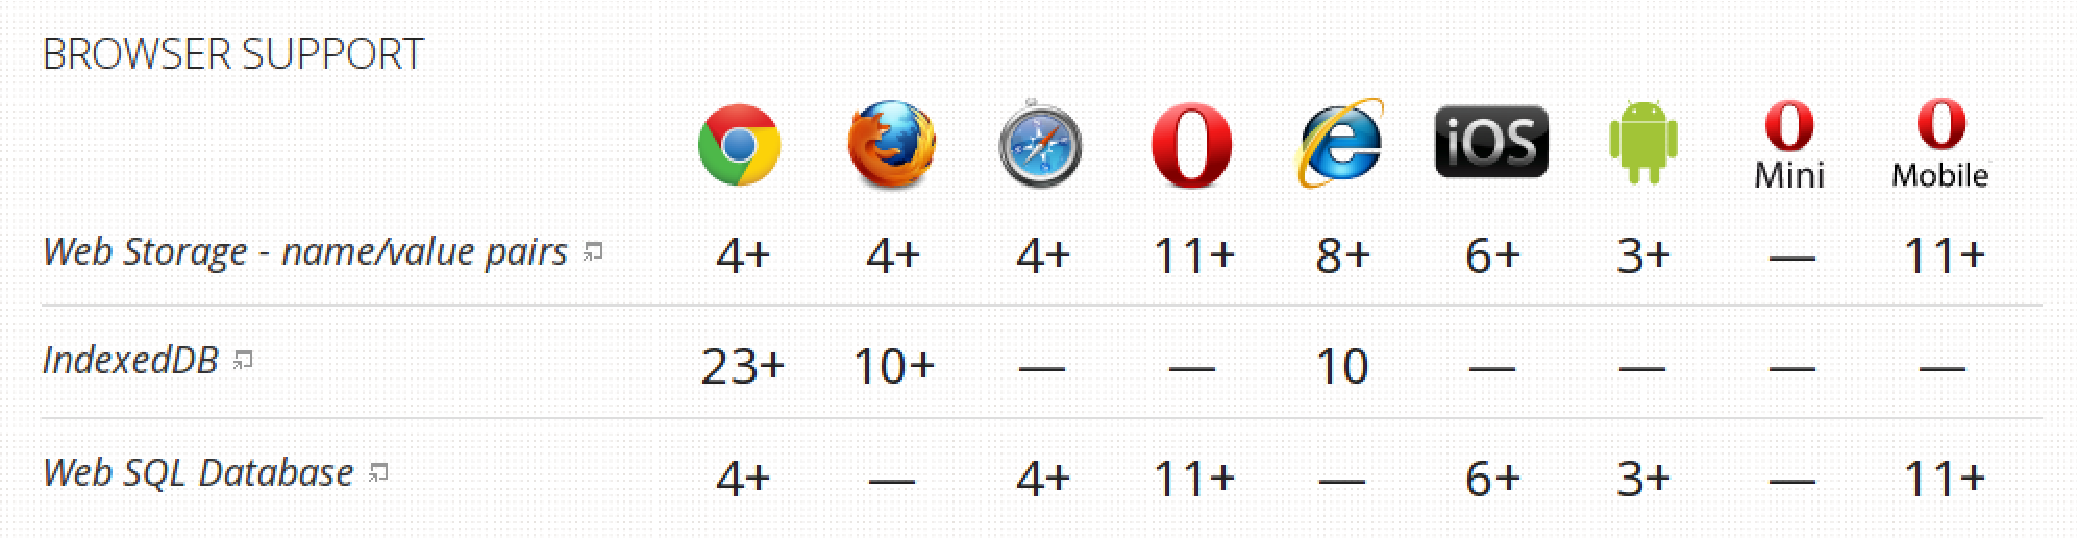
\includegraphics[width=\textwidth,height=\textheight,keepaspectratio]{./Figures/storage_browser_compatibility.pdf}
    \rule{35em}{0.5pt}
  \caption[Storage Browser Kompatibilität]{Browser-Kompatibilität der unterschiedlichen Storage-Technologien}
  \label{fig:storage_browser_compatibility}
\end{figure}
Abbildung \ref{fig:storage_browser_compatibility} zeigt, welche der vorgestellten Techologien aktuell in welchen Browsern unterstützt werden. Wie man sieht, wird bisher nur der Web-Storage flächendeckend und insbesondere auch in mobilen Browsern unterstützt. Vor allem Mozilla hat sich sehr stark gegen Web SQL und für die Verwendung von IndexedDb ausgesprochen und unterstützt auch nur noch die letztere Technologie. Gegen diese Entscheidung gibt es aufgrund der im Gegensatz zu Web SQL bedeutend komplexeren API und der komplizierten Systementwicklung auf Basis von IndexedDb eine Menge Widerspruch (vgl. \cite{Ranganathan2010}). Momentan sieht es aber danach aus, dass ob IndexedDb zu einer W3C-Recommendation wird, während Web SQL nur von einzelnen Browserherstellern unterstützt wird.

Anforderung \reqref{requirementOfflineWork} fordert, dass der Anwender zumindest rudimentär mit dem System arbeiten kann, auch wenn keine Verbindung zu dem Backend besteht. Hierfür ist es notwendig, dass vom Anwender erstellte Daten und Änderungen im Browser vorgehalten werden, damit sie bei einer Wiederherstellung der Konnektivität synchronisiert werden können. Für die Umsetzung dieser Anforderung wurde in dieser Arbeit eine Entscheidung für den Web-Storage und gegen Web-SQL und die IndexedDb-API getroffen. Ein Grund dafür ist, dass der Web-Storage, wie in Abbildung \ref{fig:storage_browser_compatibility} deutlich wird, momentan die größte Verbreitung in aktuellen und insbesondere mobilen Browsern genießt. Insbesondere für Web-SQL ist hier in Zukunft auch keine Verbesserung zu erwarten. Des Weiteren ist die Erstellung einer Applikation auf IndexedDb- und Web-SQL-Basis deutlich komplexer als auf Basis von Web-Storage, welcher für das einfache Hinterlegen von zu synchronisierenden Daten ausreicht. Durch seine einfachen Schlüssel-/Wertpaare ist er in der Umsetzung und Pflege bedeutet einfacher zu Handhaben als die anderen beiden Systeme. In Bezug auf IndexedDb ist es außerdem problematisch, dass sich die API noch nicht in einem finalisiertem Zustand befindet und noch größere Änderungen mit neuen Browserversionen zu erwarten sind.

\subsection{Online-/Offline-Erkennung}\label{section:online_offline_erkennung}
Anforderung \reqref{requirementCheckOnlineStatus} fordert, dass das System seinen Onlinestatus kennen und bemerken muss, wenn sich dieser ändert. In aktuellen Browsern existiert eine API, die es dem System erlaubt zu erkennen, ob eine Verbindung mit dem Internet besteht oder nicht. Zum einen gibt es die Eigenschaft \texttt{onLine} des globalen \texttt{navigator}-Objektes. \texttt{navigator.onLine} gibt true, wenn eine Netzwerkverbindung besteht und ansonsten \texttt{false}. Zum anderen wird bei Änderung des Online-/Offline-Zustandes ein Event aus gelöst, für welches im Code Listener definiert werden können:
\begin{lstlisting}
document.body.addEventListener("online", function () {...} 
document.body.addEventListener("offline", function () {...}.
\end{lstlisting}          
Diese in den Listenern definierten Callbacks werden bei einem Wechsel von online zu offline oder umgekehrt ausgeführt. Es ist jedoch zu beachten, dass unterschiedliche Browserhersteller "`offline"' unterschiedlich definieren. Aktuell wechselt zum Beispiel Chrome bei Verlust der Internetverbindung in den Offline-Modus, im Firefox muss dieser Modus explizit vom User angeschaltet werden (vgl. \cite{MozBug2011}).

\section{Kommunikation in Mashup-Anwendungen}\label{section:kommunikation_in_mashup_anwendungen}
Die Anforderungen \reqref{requirementAggregator} und \reqref{requirementUsageInBrowser} verlangen, dass das System einen Aggregator, also eine Mashup-Anwendung (siehe \ref{section:mashup_anwendungen}) darstellt, der unterschiedliche Systeme in aktuellen Browsern zusammenfasst. Des Weiteren soll der Nutzer in einer Art Dashboard Informationen über den Zustand der einzelnen Widgets erhalten (\reqref{requirementDashboard}). Dies erfordert, dass die Widgets in der Lage sind mit der Hauptapplikation zu kommunizieren. Die Widgets selber werden wie in Abschnitt \ref{section:widget_frameworks} beschrieben von einer Wookie-Instanz, also von einem anderen Server als die Hauptapplikation ausgeliefert. Zusammengenommen zieht dies Probleme mit Sicherheitsrichtlinien innerhalb der Browser nach sich. Dieses Kapitel behandelt diese sogenannte Same-Origin-Policy und stellt Lösungswege vor, wie trotz der gegebenen Einschränkungen eine Mashup-Anwendung funktionieren kann.

In einer Mashup-Anwendung müssen mehrere System miteinander kommunizieren. Auch und insbesondere im Hinblick auf eine einfache Erweiterbarkeit (Anforderung \reqref{requirementExtensibility}) ist es von Vorteil, wenn die Bestandteile der Anwendung für ihre Anfragen einen ähnliches Prinzip verwenden. Bei der Verwendung eines gemeinsamen Interfaces würde sich die Interoperabilität zwischen den Teilanwendungen erhöhen Entwicklern das Hinzufügen neuer Anwendungen zu der Anwendung beträchtlich erleichtern. In den letzten Jahren ist hierfür das REST-Prinzip immer weiter in den Fokus gerückt, welches ebenfalls in diesem Kapitel vorgestellt wird.
% 
\subsection{Same-Origin-Policy}\label{section:same_origin_policy}
Moderne Browser benutzen als Teil ihres Sicherheitskonzeptes die Same-Origin-Policy. Diese bewirkt, dass Sprachen, die auf Client-Seite ausgeführt werden (wie Javascript), nicht die Möglichkeit haben, Requests, also Anfragen, an einen anderen Zielpunkt als ihrem Ursprung zu starten (vgl. \cite{Ruderman2008}). Diese Policy wird also lediglich bei Zugriff auf URLs mit der selben Domain und dem selben Port, wie die URL von der die Seite geladen wurde, erfüllt. Das bedeutet, dass ein Skript auf \path{http://sop.example.com/directory1} Requests an \path{http://sop.example.com/directory2} starten kann, nicht jedoch an \path{http://example.com/directory2} (unterschiedliche Domain) oder an \path{http://sop.example.com:8080/directory2} (unterschiedlicher Port). Ausgenommen ist hierbei das in eine Seite eingebettete Laden von Ressourcen. Hierzu gehören externe Inhalte, die über iframes geladen werden aber auch externe Javascript-Dateien (über $<$script$>$...$<$/script$>$ Tags) und Medienressourcen wie Bilder und Videos. Des Weiteren ist es auch möglich Formulare an andere Zielpunkte als den Ursprung abzuschicken. Diese Einschränkung hat also primär Auswirkungen auf das Absenden von XMLHttp-Requests, also auf normale Ajax-Requests.

Die Same-Origin-Policy ist sehr sinnvoll um beispielsweise gefährlichem Javascript-Code das Ausspähen privater Daten zu verhindern. Sie erschwert jedoch die Entwicklung moderner Ajax-Anwendungen und insbesondere die Entwicklung von Mashup-Applikationen wie PLEs, welche prinzipiell so aufgebaut sind, dass sie ihre Inhalte und Ressourcen aus unterschiedlichen Quellen beziehen. In einer PLE wie in dieser Arbeit beschrieben, werden die Widgets von einem Widget-Container wie Wookie (siehe Abschnitt \ref{section:widget_frameworks}) ausgeliefert und besitzen dadurch auch die Domain des Widget Containers als Origin. Arbeiten diese Widgets nun aber nicht nur lokal beim Client, sondern benötigen für ihre Funktionalität auch externe Server, so müssen sie in der Lage sein XMLHttp-Requests an diese zu senden. Aus diesem Grund wurde der Mechanismus des Cross-Origin Resource Sharing (CORS) (vgl. \cite{vanKesteren2012}) eingeführt. Dieser erlaubt es unter bestimmten Bedingungen und Einschränkungen die Same-Origin-Policy zum umgehen.

\subsubsection*{CORS}
Wenn Cross-Origin Resource Sharing benutzt wird, kann der Server so konfiguriert werden, dass er Anfragen von anderen Origins erlaubt und angibt welche Header in diesen Anfragen vorkommen dürfen. Ein einfacher CORS-Request vom Client zum Server sieht wie folgt aus (Workflow analog zu \cite{Hossain2012}):
Der Client sendet eine Cross-Origin-Anfrage mit einem Origin Header an den Server:
\begin{lstlisting}
GET /cors HTTP/1.1
Origin: http://api.bob.com
Host: api.alice.com
Accept-Language: en-US
Connection: keep-alive
User-Agent: Mozilla/5.0...
\end{lstlisting}
Anschließend antwortet der Server mit:
\begin{lstlisting}
Access-Control-Allow-Origin: http://api.bob.com
Access-Control-Allow-Credentials: true
Access-Control-Expose-Headers: FooBar
Content-Type: text/html; charset=utf-8
\end{lstlisting}
Alle für den CORS-Request relevanten Header beginnen mit Access-Control. \texttt{Access\allowbreak -Control\allowbreak -Allow\allowbreak -Origin} bedeutet, dass der Server eine Cross-Origin-Anfrage von dem angegebenen Origin erlaubt, \texttt{Access\allowbreak -Control\allowbreak -Allow\allowbreak -Credentials: true} besagt, dass in diesem Request auch Cookies erlaubt sind. Möchte der Client Zugriff auf Nicht-Standard-Header aus der Antwort des Servers, müssen diese in \texttt{Access\allowbreak -Control\allowbreak -Expose\allowbreak -Headers} angegeben werden.

Sollte der Client einen Request mit einer anderen Methode als \texttt{GET} oder \texttt{POST} (siehe \ref{section:rest}) senden, reicht dieser einfache Workflow nicht aus. In diesem Fall muss vor der eigentlichen Anfrage ein so genannter "`Preflight-Request"' ablaufen, welcher verifiziert, dass der Server diese Methode als CORS-Request erlaubt.

Diese Methodik erlaubt also, das Widgets von einem Widget-Container ausgeliefert werden, dadurch einen anderen Origin bekommen und trotzdem Requests an ihr eigentliches Backend senden zu können. Damit ist sie ein essentieller Baustein für den Aufbau von Mashup-Anwendungen im Internet.

\subsubsection*{Postmessage}
Für die in Anforderung \reqref{requirementWidgetInformSystem} geforderte Darstellung der wichtigsten Informationen über den Zustand eines Widgets ist es notwendig, dass die Hauptapplikation Daten von den Widgets erhalten oder auslesen kann. Mashup-Anwendungen im Internet werden wie in Kapitel \ref{section:widgets} beschrieben hauptsächlich über iframes umgesetzt. Die Same-Origin-Policy aktueller Browser erlaubt aber nur, dass die Hauptanwendung nur Daten aus iframes mit der gleichen Origin ausliest. Dies erschwert den Informationsaustausch zwischen der Hauptapplikation und den Widgets beträchtlich. Aus diesem Grund wurde das "`Postmessage"'-System entwickelt, welches diese Einschränkung auf eine sichere Art und Weise umgeht. Mit Hilfe von Postmessage ist es möglich, dass sich unterschiedliche Fenster (zum Beispiel Frames) Nachrichten schicken können. Andere Fenster können Event-Listener implementieren, welche auf diese Nachrichten hören (vgl. \cite{MDN2012}). Im folgenden Listing sieht man, wie solch eine Nachricht versendet wird (aus \cite{MDN2012}):
\begin{lstlisting}
otherWindow.postMessage(message, targetOrigin);
\end{lstlisting}
\texttt{otherWindow} ist hierbei eine Referenz auf ein anderes Fenster oder einen anderen Frame, welches über Standard-DOM-Methoden zu erreichen ist. \texttt{message} ist die Nachricht selber (kann auch ein Javascript-Objekt sein) und \texttt{targetOrigin}, ist die Origin, die \texttt{otherWindow} haben muss, damit die Nachricht verschickt wird. Damit \texttt{otherWindow} die Nachricht empfängt, muss auf dieser Seite ein Event Listener implementiert werden:
\begin{lstlisting}
window.addEventListener("message", receiveMessage);
function receiveMessage(event) {
  if (event.origin !== "http://example.org:8080")
    return;
  // ...
\end{lstlisting}
Empfängt das Fenster also eine Nachricht ist es möglich auch den Origin des Senders zu prüfen, damit man nur Nachrichten aus vertrauenswürdigen Quellen bearbeitet.

Mit dieser Technik ist es möglich, dass sich Widgets bei der Hauptapplikation registrieren und ihr Informationen, z.B. über die Anzahl der vorhandenen Einträge, zukommen lassen. Diese Informationen kann die Hauptapplikation dann für den Anwender aufbereiten und darstellen, so dass sich Anforderung \reqref{requirementWidgetInformSystem} erfüllen lässt.

\subsection{REST}\label{section:rest}
REST (Representational State Transfer Protocol), ist ein Architekturstil, welcher versucht 
\begin{quotation}
für statische Inhalte und dynamisch berechnete Informationen, die ein globales, gigantisches Informationssystem bilden, ein einheitliches Konzept zu definieren. (vgl. \cite{tilkovrestchapter2})
\end{quotation}
Systeme, die nach diesem Konzept entwickelt wurden befolgen die im folgenden oberflächlich beschriebenen Prinzipien. Dies führt im Idealfall zu positiven Eigenschaften, wie der losen Kopplung von Systemen, dem Vorhandensein allgemeiner Interfaces und einer dadurch erhöhten Interoperabilität, Wiederverwendbarkeit und Erweiterbarkeit führt (vgl.\cite{tilkovrestchapter2}).

Theoretisch ist es möglich ein beliebiges REST-konformes Protokoll zu entwickeln und anzuwenden, normalerweise wird jedoch das im Internet dominierende HTTP-Protokoll für die Umsetzung benutzt. Der Grund hierfür ist, dass dieses Protokoll bei korrekter Anwendung die wichtigsten Anforderungen des REST-Prinzips erfüllt und schon im Hinblick auf diesen Architekturstil entworfen wurden (einer der Hauptbeteiligten am Entwurf der HTTP-Spezifikation, Roy Fielding, hat mit seiner Dissertation :"`Architectural Styles and the Design of Network-based Software Architectures"'\footnote{\url{http://www.ics.uci.edu/~fielding/pubs/dissertation/top.htm}} das REST-Prinzip entwickelt). 

Nach \cite{tilkovrestchapter2} ergeben sich für REST fünf Grundprinzipien:
\begin{enumerate}
 \item\label{enumerate_rest_principles:1} Ressourcen mit eindeutiger Identifikation
 \item\label{enumerate_rest_principles:2} Verknüpfungen Hypermedia
 \item\label{enumerate_rest_principles:3} Standardmethoden
 \item\label{enumerate_rest_principles:4} Unterschiedliche Repräsentationen
 \item\label{enumerate_rest_principles:5} Statuslose Kommunikation
\end{enumerate}

In einem REST-Entwurf wird nach Entitäten gesucht, welche auf Ressourcen abgebildet werden. Dies ähnelt einem objektorientierten Entwurf, es gibt hierbei jedoch zwei wichtige Unterschiede. Es werden den Ressourcen keine neuen Methoden oder Verben hinzugefügt, sondern es werden nur die Standardmethoden genutzt. Um trotzdem keine Einschränkung in der Mächtigkeit dieses Prinzips in Kauf nehmen zu müssen, werden mehr Ressourcen hinzugefügt, als es eigentlich Entitäten gibt. Punkt \ref{enumerate_rest_principles:5} in den obigen Forderungen bedeutet, dass der Server keinerlei Session Informationen über den User speichert. Dies hat zur Folge, dass beispielsweise der Warenkorb in einem Shop ebenfalls als Ressource angelegt werden muss. Der Vorteil von dieser Vorgehensweise ist der, dass somit z.B. auch Lesezeichen auf einen Warenkorb angelegt werden können. Zusätzlich gibt es beispielsweise noch neben den Primärressourcen, welche einzelnen Entitäten abbilden, Listenressourcen welche für die Auflistung einer Menge von Ressourcen eines bestimmten Typen genutzt werden (vgl. \cite{tilkovrestchapter4}). Im Internet besteht bereits ein eindeutiges System für die öffentliche Vergabe von Ressourcen-Identifizierern: die URI(Uniform Resource Identifier, z.B. \path{http://example.com/accounts/5?paginate=1&page=3}). URIs stellen einen allgemein verfügbaren Namensraum zur Verfügung, in dem Ressourcen identifiziert werden können. Punkt \ref{enumerate_rest_principles:4} fordert, dass Ressourcen in unterschiedlichen Repräsentationen ausgeliefert werden können. So ist es beispielsweise möglich, dass es eine maschinenlesbare Repräsentation im XML Format und eine für Menschen im Browser darstellbare Repräsentation im HTML Format gibt. Der Client kann über einen Accept-Header ein bestimmtes Format anfordern.
Möchte man zum Beispiel einen Kunden über eine Ressource abbilden könnte der Identifizierer \path{http://example.com/customers/4} sein. Eine Anfrage der Darstellung kann dann als einfacher HTTP-Request abgeschickt werden:
\begin{lstlisting}
GET /customers/4 HTTP/1.1
Host: example.com
Accept: application/xml 
\end{lstlisting}
Der Server gibt in mit einem Statuscode (hier 200 OK) zurück, ob die Anfrage erfolgreich war und fügt dann die gewünschte Repräsentation der Ressource an:.
\begin{lstlisting}
HTTP/1.1 200 OK
Content-Type: text/xml; charset=utf-8
Content-Length: ...

[XML spezifische Kopfzeilen]
<customer href="./customers/4">
  <name>Roman Sachse</name>
  <orders>
    <order>
      <delivered>true</delivered>
      <link>http://example.com/orders/54>
\end{lstlisting}
In der Antwort des Server finden sich Links auf weitere mit dem Kunden verknüpfte Ressourcen. Dies ist eine Umsetzung des Hypermedia-Prinzip, welches für ein vollkommenes REST-System fordert (vgl. \cite{tilkovrestchapter2}), dass sich Client ab einem Startpunkt aus nur durch das Verfolgen Links durch das gesamte System bewegen könnte. Eine Listenressource würde man über \path{http://example.com/customers} abfragen, die Antwort könnte dann in XML Verweise auf die einzelnen Customer erhalten. Zusätzlich könnten bei gewünschter Paginierung der Ergebnisse (beispielsweise über Query-Parameter wie \path{http://example.com/customers?page=2} noch Links auf die vorherige und nächste Seite zurückgegeben werden.

Wie man in der obigen Anfrage sieht, wird eine Anfrage mit dem Verb GET an den Server geschickt. Das HTTP-Protokoll stellt unterschiedliche Standardmethoden bereit, mit denen ein Client eine Ressource Abfrage kann. Der Vorteil bei der Nutzung dieser Standardmethoden liegt darin begründet, dass mit ihnen ein Interface existiert, mit dem alle Ressourcen abgefragt werden können und die ein Server für alle Ressourcen versteht. Sollte dies einmal nicht der Fall sein, kann der Server mit einer Fehlermeldung im Sinne von "`Methode wird für diese Ressource nicht unterstützt"' antworten. Für Methoden gibt es zwei wichtige Merkmale. Sie können sicher und/oder idempotent sein (vgl. \cite{tilkovrestchapter5}). Sicher bedeutet in diesem Fall, dass ein Request auf eine Ressource mit dieser Methode keine Seiteneffekte hat, d.h. die Ressource nicht verändert wird. Idempotent meint, dass eine Methode auf sich selbst angewandt wieder das selbe Ergebnis liefert (mathematisch: f(x) = f(f(x))). Idempotenz ist in diesem Umfeld ein wichtiges Konzept, da es immer möglich ist, dass der Client durch unerwartete Probleme (Verbindungsabbruch etc.) keine Antwort vom Server auf seine Anfrage erhält. Bei idempotenten Methoden kann er seine Anfrage einfach noch einmal stellen, ohne befürchten zu müssen, dass auf dem Server, ein Zustand eintritt, den er nicht erwartet hat. HTTP stellt acht Methoden bereit, wobei hier nur die wichtigsten fünf kurz vorgestellt werden (vgl. \cite{tilkovrestchapter5}:
\begin{enumerate}
 \item mit \texttt{GET} fordert der Client eine Repräsentation (in einem zu spezifizierendem Format) einer Ressource an. sicher: ja, idempotent: ja
 \item \texttt{PUT} weist einen Server an eine Ressource zu aktualisieren und wenn nicht vorhanden zu erstellen. sicher: nein, idempotent ja 
 \item \texttt{POST} weist einen Server an eine Ressource zu erstellen (wird an Listenressource gesendet). sicher: nein, idempotent: nein
 \item \texttt{DELETE} weist einen Server an eine Ressource zu löschen. sicher: nein, idempotent: ja
 \item \texttt{OPTIONS} liefert Metadaten für eine Ressource - z.B. Allow-Header, welche angeben, welche Methoden/Header akzeptiert werden, wichtig für CORS (siehe \ref{section:same_origin_policy})
\end{enumerate}

Um zu den Customer-Ressourcen aus dem obigen Beispiel also einen Kunden hinzuzufügen, müsste man einen POST-Request an die Listenressource \path{http.example.com/customers} senden. Ein einzelner Kunde kann mit einem GET-Request an die Primärressource \path{http.example.com/customers/4} ausgelesen werden. PUT oder DELETE würden die Ressource dementsprechend aktualisieren oder löschen

GET und POST sind die am häufigsten genutzten Methoden. Der Grund hierfür ist, dass diese beiden Methoden der normale Weg eines Browser sind mit einem Server zu kommunizieren. Jeder direkte Aufruf einer URI über einen Browser sendet eine GET-Anfrage an einen Server. Die im Web häufig anzutreffenden Formulare werden meist über eine POST-Anfrage abgeschickt. So werden diese beiden Methoden ausserhalb von Anwendungen, die dem REST-Prinzip folgen, auch für alle anderen Anfragen benutzt, so dass man sich bei diesen Anwendungen nicht sicher sein kann, ob ein GET-Request an eine URI nicht ein Ändern oder Löschen der Ressource zur Folge hat (man betrachte beispielsweise die URI: \path{http://example.com/customers/5?action=delete}).

Wird eine Anwendung im Hinblick auf REST-Prinzipien umgesetzt, so vereinfacht dies die Erweiterung dieses Systems beträchtlich (Anforderung \reqref{requirementExtensibility}). Insbesondere für Mashup-Anwendungen bei denen unterschiedliche Systeme miteinander kommunizieren müssen, ist beispielsweise die Nutzung eines gemeinsamen Methodeninterfaces sehr hilfreich, da nicht für jedes System ein weiteres Kommunikationsprotokoll erstellt werden muss. Das System dieser Arbeit hat noch die zusätzliche Anforderung den Anwender in die Lage zu versetzen auch offline zu arbeiten (Anforderung \reqref{requirementOfflineWork}). Wenn das System für das Speichern der Daten im Browser ebenfalls auf REST aufsetzt, wird es mit relativ wenig Aufwand möglich sein weitere offline fähige Widgets für unterschiedliche Services zu erstellen. Die Art des Services ist dabei egal, solange er in der Lage ist einfache REST-Anfragen zu verstehen, zu verarbeiten und standardkonform auf sie zu antworten. Für den Entwickler wird es in diesem Fall vollkommen transparent sein, ob sich das System in einem online oder offline ist. Er kann unabhängig von dem Zustand die Daten ohne zu implementierende Fallunterscheidungen speichern und abfragen.

\section{Eine PLE auf dem USB-Stick}\label{section:ple_auf_usb}
Anforderung \reqref{requirementUsbStick} fordert die Möglichkeit das System auf unterschiedlichen Rechnern zu benutzen und die Daten offline zwischen diesen Rechnern auszutauschen. Da alle systemrelevanten Daten im Browser hinterlegt werden (Application-Cache (siehe \ref{section:appcache}) und Web-Storage (siehe \ref{section:offline_storage}), ist es notwendig die gesamte Browserinstallation zwischen unterschiedlichen Rechnern hin und herbewegen zu können. Der einfachste Weg hierfür ist die Installation des Browsers auf einem portablen Speichermedium wie einem USB-Stick. Hierfür gibt es beispielsweise die Open-Source-Anwendung \href{http://portableapps.com/}{PortableApps}\footnote{\url{http://portableapps.com/}}, die genau dies erlaubt wodurch diese Anforderung relativ leicht zu erfüllen ist. 

\section{Ähnliche Systeme}\label{section:aehnliche_systeme}
Wie in Kapitel \ref{chapter:Kapitel2} beschrieben gibt es zwei unterschiedliche Arten vom E-Learning Systemen. Lern-Management-Systeme (LMS) und Personal Learning Environments (PLE). Vertreter der klassischen LMS sind beispielsweise \href{https://moodle.org/}{Moodle}\footnote{\url{https://moodle.org/}}, \href{http://www.sakaiproject.org/}{Sakai}\footnote{\url{http://www.sakaiproject.org/}}, \href{http://www.adrenna.com/}{Adrenna}\footnote{\url{http://www.adrenna.com/}} oder \href{http://www.blackboard.com/}{Blackboard}\footnote{\url{http://www.blackboard.com/}}. Diese Systeme verfolgen den sehr kurszentrierten Ansatz klassischer Lern-Management-Systeme und widersprechen damit dem PLE-Ansatz. Es gibt, insbesondere für Moodle, Bestrebungen PLE-Funktionalitäten in das System mit aufzunehmen. Die Ansätze hierfür reichen von der Idee einfach allen Studenten die Rechte zu geben eigene Kurse anzulegen\footnote{\url{https://moodle.org/mod/forum/discuss.php?d=124174}}, so dass sie sich einen eigenen Arbeitsplatz zusammenzustellen können, bis hin zu dem Versuch Services aus dem Web 2.0 über Widgets mit dem Moodle-Kern kommunizieren zu lassen (vgl. \cite{Penalvo2011}). Letzteres mündete in die Entwicklung des \href{http://www.moodbile.org/}{Moodbile}\footnote{\url{http://www.moodbile.org/}} Systems, welches das Ziel hat mobile Anwendungen mit Hilfe von W3C-Widgets und Wookie in Moodle einzubinden. Dieses Projekt wird jedoch seit einiger Zeit nicht weiterentwickelt und ist nicht kompatibel zu aktuellen Moodle-Versionen. Nach \cite{Penalvo2011} befindet sich das Ziel PLEs mit LMS zu verbinden und integriert miteinander arbeiten zu lassen noch in weiter Ferne. Systeme wie Blackboard oder Adrenna bauen auf aktuellen Webtechnologien auf und geben trotz ihres institutszentrierten Charakters dem Anwender die Möglichkeit sich mit Services wie Youtube oder Twitter zu verbinden. Beide Systeme müssen jedoch von einem Institut installiert und den Anwendern zu Verfügung gestellt werden, können also nicht von Anwendern außerhalb des Institutes genutzt werden. Sie bieten zwar APIs zur Implementation neuer Funktionalitäten, ihr Quellcode ist jedoch nicht freigeben und unterliegt proprietären Lizenzen.

In den Bereich der PLEs fallen Systeme, die es dem Anwender erlauben sich sein eigenes System aus Widgets zusammenzubauen, also wirklich als Informationsaggregatoren fungieren. Die zwei wichtigsten und verbreitetsten Vertreter dieser Art Anwendungen sind das von Google entwickelte \href{http://www.google.de/ig}{iGoogle}\footnote{\url{http://www.google.de/ig}} und \href{http://www.netvibes.com}{Netvibes}\footnote{\url{http://www.netvibes.com}}. Beide Systeme verfolgen den Ansatz einer personalisierbaren Homepage. Es ist möglich Widgets für die unterschiedlichsten Services aus einer Widget-Datenbank auszuwählen und dem System zuzuordnen. Die Widgets können innerhalb des Systems unterschiedlichen frei definierbaren Arbeitsflächen sogenannten Workspaces oder Tabs zugewiesen und dort per Drag and Drop angeordnet werden. Als Widget-Format benutzt Netvibes die eigens entwickelte "`Universal Widget API"' (\href{http://dev.netvibes.com/doc/uwa}{UWA}\footnote{\url{http://dev.netvibes.com/doc/uwa}}), welche erlaubt Widgets auf Basis von HTML, XML, und Javascript zu entwickeln. Für iGoogle hat Google die sogenannten \href{https://developers.google.com/gadgets/}{Google Gadgets}\footnote{\url{https://developers.google.com/gadgets/}} entworfen. Die in Abschnitt \ref{section:opensocial_gadgets} vorgestellten OpenSocial Gadgets basieren zum Großteil auf der Google Gadgets Spezifikation. Zusätzlich zu den eigenen Widgets werden auf der iGoogle Startseite neben einem Standardsuchfeld für die Google Suche, nicht entfernbare Direktlinks zu anderen Google-Services wie Calender, Google Drive oder Google+ angeboten. Weder das Netvibes noch das iGoogle Grundsystem stehen als Open Source im Quellcode zur Verfügung. Beide Systeme sind kostenlos, zusätzliche Funktionen (insbesondere für Business Anwendungen) können bei Netvibes für 499 Dollar im Monat dazu gebucht werden. Google hat angekündigt das iGoogle-System zu Gunsten des Chrome App Shops oder Google Play Marktplatzes für Android-Systeme zum 1. November 2013 abzuschalten (vgl. \cite{Google2012}).

In ihrer Funktionalität und Arbeitsweise ähneln Netvibes und iGoogle sehr dem in dieser Arbeit zu entwickelnden System. Beide Systeme besitzen jedoch keine expliziten Funktionalitäten zum Offline-Arbeiten. Netvibes erlaubt es einzelne Artikel zum Beispiel in einem Newsfeed als "`zum später Lesen"' zu markieren und herunterzuladen. Es gibt jedoch weder Möglichkeit die Seite erneut zu laden, wenn keine Internetverbindung besteht, noch eine Möglichkeit offline weiterzuarbeiten und vorgenommene Änderungen bei einer erneuten Verbindung zu synchronisieren. 